\chapter{相关研究}



\section{基于编码结构优化的数据修复技术}

在多个同时发生的故障事件中,单个节点故障的恢复率可达到$98\%$\cite{rashmi2014hitchhiker,xia2015tale}。因此,减少单一故障修复所产生
的延迟对于提高系统性能是至关重要的。\citet{dimakis2007benefits,dimakis2010network}提出了再生码RGC,它可以在存储开销和修复故障节点所需的数据量之间
取得良好的均衡。另一方面,处于最小存储的再生码均衡点的MSR(Minimum Stroage Regenerating)对于大部分纠删码来说是最优的替代选择,因为MSR可以在
最小存储开销下实现最佳修复成本和最大距离可分MDS的特性。MDS属性意味着只要故障块数小于或等于校验块数,那么数据就可以被恢复。然而,MSR码有一些缺点。
(1)大多数现有的MSR码不是系统码,只在编码后存储奇偶校验块信息,因此造成了很高的计算开销;
(2)许多纠删码的存储开销超过系统存储量的2×倍,因此在实际存储系统中没有用处不大;
(3)存储开销低于系统存储量的2×倍的码不仅需要复杂且容易出错的代码策略,而且还需要很高资源的开销。
对于这些问题,Butterfly\cite{pamies2016opening}可以在低存储开销(低于2×倍)的情况下具有实际应用价值的MSR码,
是一种系统化的码,读请求可以直接得到数据而不需要任何解码操作。然而,Butterfly最多只能容忍两个块的故障,因此不能达到高可靠性的标准。
此外,它还存在一个成簇的子包,它将块分成小的片段(最小的编码元素),导致编解码操作中会损失块的位置数据,还会产生数据读取和传输的高通信成本。

\citet{ye2017hybrid}提出了Hybrid-RC利用Butterfly码来对MSR进行优化改进,理论上它是可以在低存储开销和低修复带宽之间取得最优均衡的纠删码。Hybrid-RC使用Butterfly
作为分组校验编码的编码策略,使用伽罗瓦运算进行全局校验码的计算从而保持存储系统的可靠性。与LRC相比,在相同的存储开销下,Hybrid-RC在处理单块故障
恢复时有着更多的数据块参与。每个块的I/O消耗相对减少且数据传输是高度并行的,从而达到了良好的平衡。

Hybrid-RC由三个标准化参数组成,$k,l,g$,记为$A(k,l,g)$。
一个条带中有$k$个数据块和$l+g$个校验块,其中$g$个全局校验块通过对所有数据块进行伽罗瓦运算求出。Hybrid-RC将$k$块数据分成$\frac{l}{2}$个组,其中
$l$必须为偶数。当$k$不能被$\frac{l}{2}$整除时且余数为$r$时,那么第0到第$r-1$组应该包含$\left\lceil\frac{2 k}{l}\right\rceil$个块并且每个块被分成了
$2^{\left(\left\lceil\frac{2 k}{l}\right\rceil-1\right)}$个片段。如果不同的组的切片数不同,那么从第$r-1$个到第$\frac{l}{2}-1$个组
应该加倍以保证每个块的存储消耗保持一样。例如,考虑$A(7,4,1)$的Hybrid-RC码,节点中的每个块大小为1GB。第一个组包含4个数据块和2个校验块,所以每个块
有8个切片且每个切片大小为0.125GB。但是,第二个组只有3个数据块,因此每个块有4个切片。为了两个组能保持同样的块大小,第二组的每个块大小需要为0.25GB。
总的来说,不同组的奇偶块构建和块修复是相互独立的。
对于全局编码或修复,最小的操作元素是相同的。因此,不同数量或大小的切片对全局奇偶校验计算是没有影响的。在一个$(k,l,g)$的Hybrid-RC码中,
$D_{i,j}$表示$D_{i}(0 \leq i<k)$数据块的第$j$个数据切片。设$P_h$为垂直码,$P_b$为butterfly码,$P_{h,x}$和$P_{b,x}$分别为第$x$组的分组校验码,其中
$0 \leq x<l / 2$。类似地,第$y$个全局校验码为$P_{g,y}$,其中$0 \leq y < g$。如图~\ref{fig:con-2.1}所示的是,第二组和全局校验码的构建过程。
不同颜色的高亮表示不同元素所属相同的运算集群。

\begin{figure}[htbp]
	\centering
	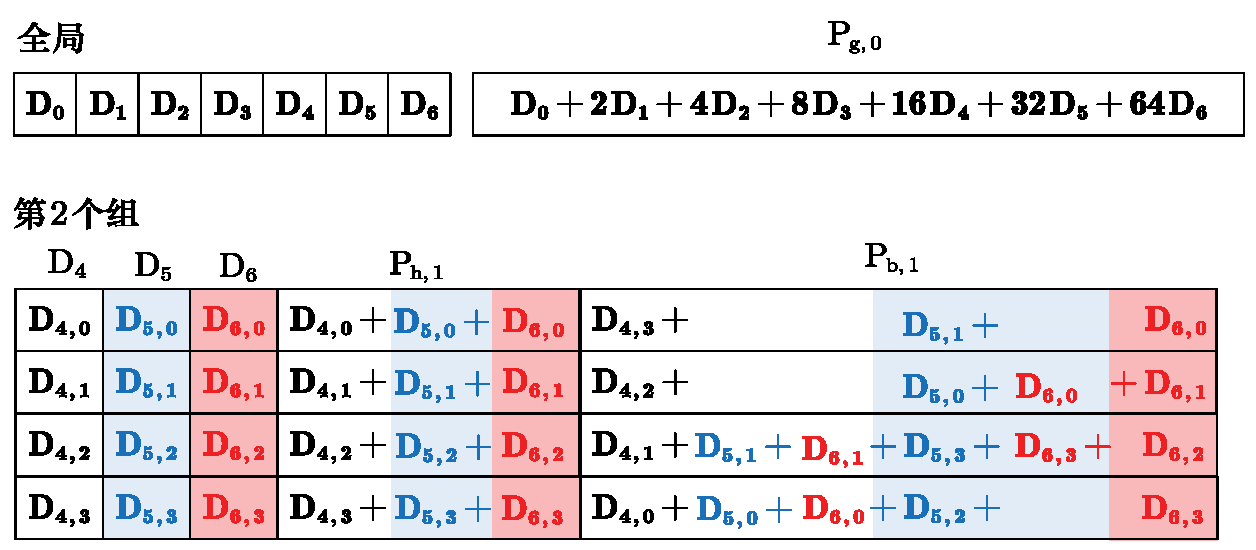
\includegraphics [scale=0.7]{figures/2.1.pdf}
	\caption{(7,4,1)Hybrid-RC}
	\label{fig:con-2.1}
\end{figure}

\citet{xie2019az},提出了在可用性区域AZ(Availability Zone)的概念,所谓AZ就是
数据中心中的一个物理隔离区域,它由几个服务器机架或数据中心的一个机柜,甚至是整个数据中心组成。
通过使用多个AZ,云存储系统可以保有高可用性,高可靠性以及低网络延时。
当前的AZ有以下三个缺点,
首先,对于基于XOR的编码,大多数基于XOR的纠删码\citep{corbett2004row,blaum1995evenodd}只能容忍两个或三个节点的故障,
这不能满足容忍AZ级节点容错能力的要求。
一些基于XOR的编码可以容忍三个以上的节点,但可扩展性却相当差\cite{zhang2015tip,huang2008star}。
第二,对于基于RS的纠删码,虽然可以提供较高的可扩展性,但修复成本(如重建I/O,修复带宽)非常高。
第三,虽然最小存储再生码\cite{vajha2018clay,ye2017explicit}可以有效地减少恢复开销,但计算复杂度比基于RS和基于XOR的代码要高得多。
基于此,他们提出了AZ-Code为AZ提供低修复开销且高可靠性的保证。AZ-Code是基于MSR码和LRC码的改进,其利用一个特定的MSR码作为LRC码的局部校验块,
用RS码生成全局校验块,通过数学分析和Hadoop系统实验分析,AZ-Code节省了高达78.24\%的修复带宽。



\section{基于调度优化的数据修复技术}

在加速节点传输的技术上,PPR\cite{mitra2016partial},RP\cite{li2017repair},TDR\cite{li2009tree}等技术充分利用各节点的带宽资源,加速
修复的速度。由于磁盘I/O和编码计算的时间开销比网络传输的要小得多\cite{li2017repair,mitra2016partial},所以优化修复数据的传输路径对修复性能的提升有着很大的意义。
对于单节点恢复,PPR和RP使用的是一种固定的树结构,而TDR技术计算的是最大生成树作为传输结构。在RP和TDR中,节点每次只执行一种任务,即将数据输送到下一个节点,
而在PPR中,部分节点并行地将数据传输到它们的专属节点。
PR和TDR没有对多节点修复进行优化,而PPR需要额外的中继节点来参与多节点的修复,同时也造成了多余的带宽消耗。
PPR和RP针对的是流量均匀的网络,
而对于TDR来说,基于的假设是:每个链路的带宽是一个常数,不受到连接到同一节点的节点数的影响。

但是在带宽不对等的环境中,
当一个节点同时接收两个或多个节点的数据时,其与每个对应的节点的实时带宽会减半或者相应比例的减少,若这样进行并行传输可能会比通过中继节点传输消耗的时间更短。
基于此,\citet{bai2019fast}提出了PPT(Parallel Pipeline Tree)通用传输
技术,根据各节点之间的带宽值构建了树状修复路径,进一步利用带宽不对等来加速单节点的修复。若PPT找不到进一步的优化,则退化到RP进行修复。
当多节点发生故障时,每个节点的数据请求需要接收所有中继节点的数据,每个中继节点将向所有请求节点发送数据。
在大多数情况下,中继节点的数量多于请求节点的数量,则整个网络的修复瓶颈则是请求节点的带宽瓶颈。
为了优化此问题,他们同时提出了一种通用解决方案,称为PPCT(Parallel Pipeline Cross-Tree),从而构建了一种交叉修复路径,
并在交叉树上并行地输送数据,进一步加快多节点修复速度,且PPT和PPCT支持基于Reed-Solomon(RS)码的实用纠删码结构。

然而,\citet{zhou2022bandwidth}发现PPT的并行传输会引发网络拥堵和带宽争夺消耗,同时会产生新的低带宽链路。基于此他们提出了SMFRepair,一种单节点多级传输的修复技术。
如图~\ref{fig:2.3}所示,在分布式存储系统中,图~\ref{fig:2.3-4}中空闲节点是非常普遍的,并且通常有足够的可用带宽。
在图~\ref{fig:2.3-1}中,$helper1$和$helper2$会异步地向$requestor$传输数据块。
而在图~\ref{fig:2.3-2}中,PPR的链接$helper2 \rightarrow helper2$的带宽很低,只有2MB/s。
通过利用链路之间的带宽差距,PPT使用并行传输来绕过低带宽的链路。
在图~\ref{fig:2.3-3}中,helper1和helper2同时向requestor发送数据块。
因为$helper1 \rightarrow requestor$的带宽为8/2=4MB/s,且$helper1 \rightarrow requestor$的带宽为5/2=2.5MB/s的带宽,
都大于$helper2 \rightarrow helper1$的2MB/s的低带宽,
所以通过新的低带宽链路可以避免带宽瓶颈问题。而在\citet{zhou2022bandwidth}的研究中,可以通过空闲节点来绕过低带宽的链接。
在图~\ref{fig:2.3-4}中,他们使用空闲节点来构建两个链接($helper2 \rightarrow $空闲节点和空闲节点$\rightarrow helper1$),
它满足两个链路带宽的倒数之和小于第三个链路带宽的倒数的条件(1/10 + 1/10 < 1/2)。
他们用这个转发链路来代替低带宽链路,且对于一个20MB的数据块,PPR需要20/2+20/8=12.5s,P
PT需要max(20/4,20/2.5)=8.0s,而SMFRepair只需要20/10+20/10+20/8=6.5s。
通过仿真实验表明,与最先进的修复技术相比,SMFRepair可以加速单节点的恢复,最高可达47.69\%,
且他们提出的多节点调度算法MSRepair可以减少多节点恢复时间33.78\%-67.53\%。

\begin{figure}[tb!]
    \centering
    \begin{subfigure}[t]{0.4\textwidth}
           \centering
           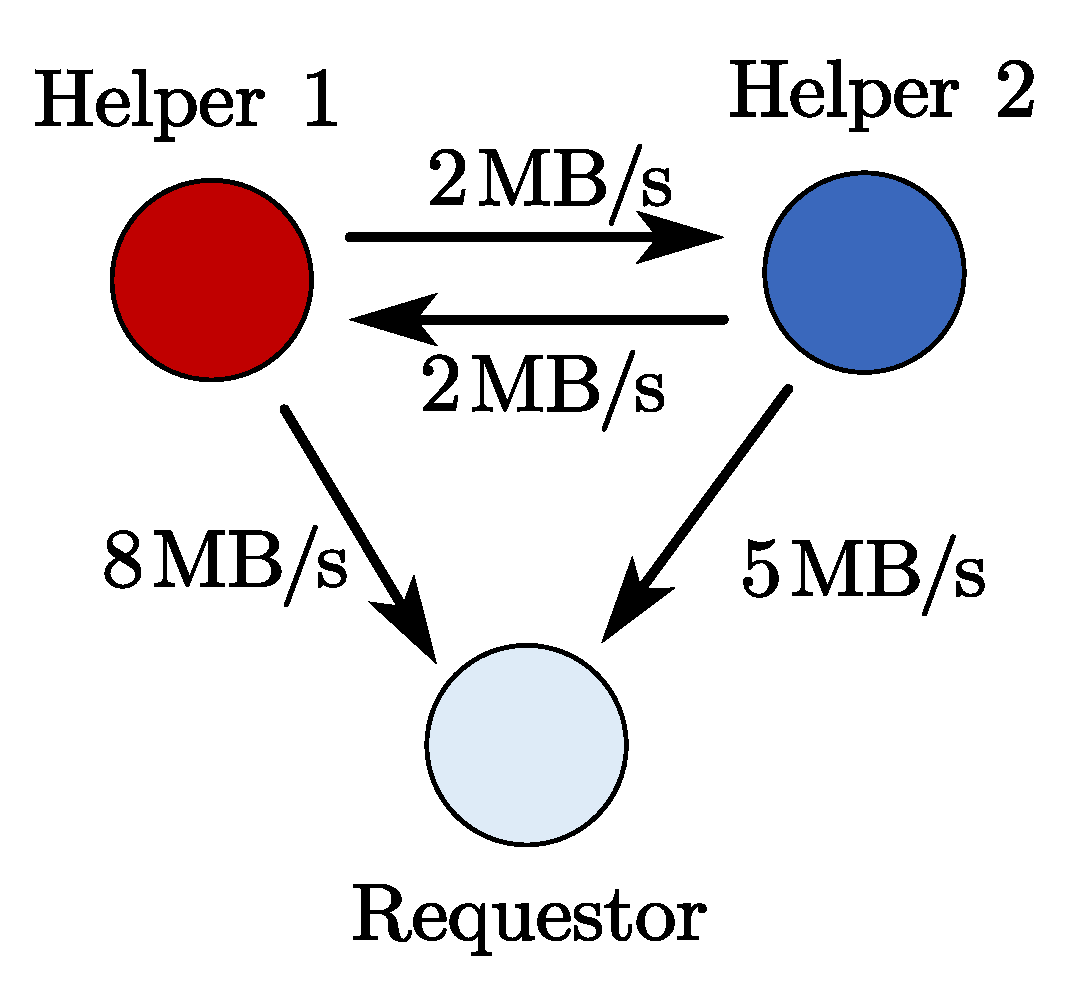
\includegraphics[scale=0.25]{figures/2.3-1.pdf}
            \caption{两个helper和一个requestor的网络模型}
            \label{fig:2.3-1}
    \end{subfigure}
    \begin{subfigure}[t]{0.4\textwidth}
            \centering
            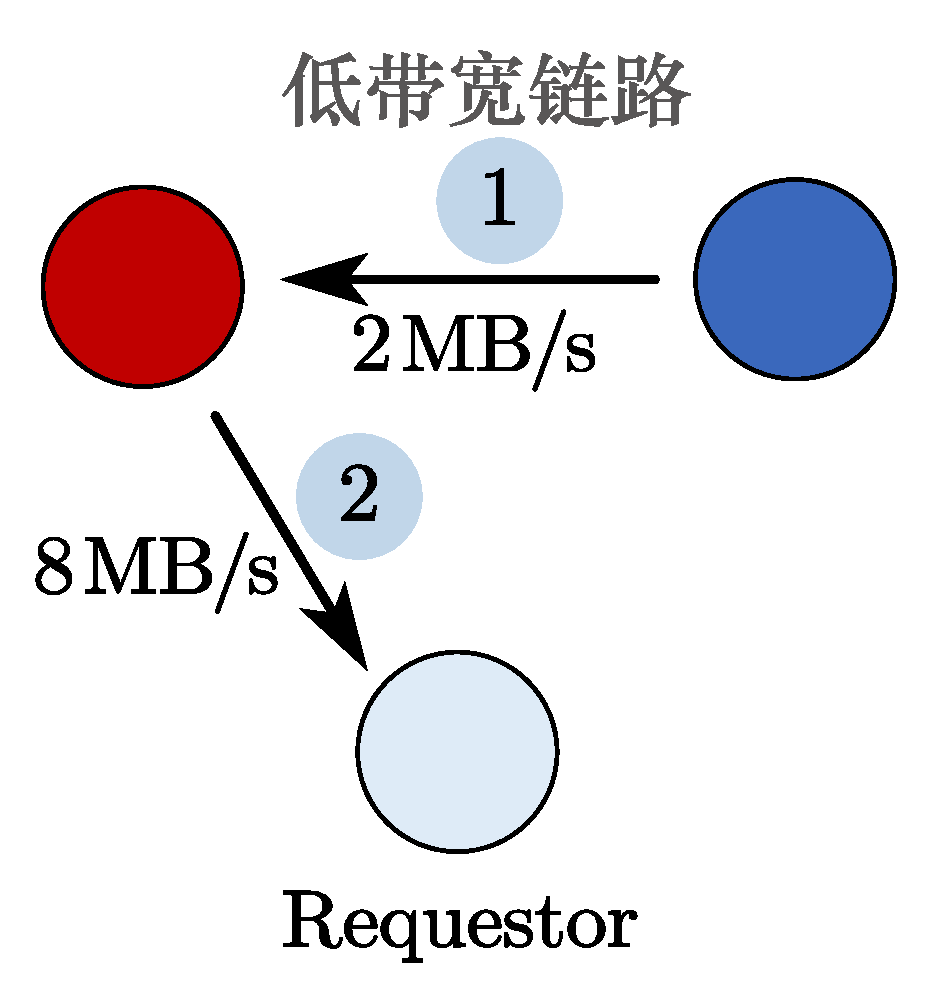
\includegraphics[scale=0.25]{figures/2.3-2.pdf}
            \caption{PPR: helper2到helper1是低带宽链路}
            \label{fig:2.3-2}
    \end{subfigure}
    \begin{subfigure}[t]{0.4\textwidth}
            \centering
            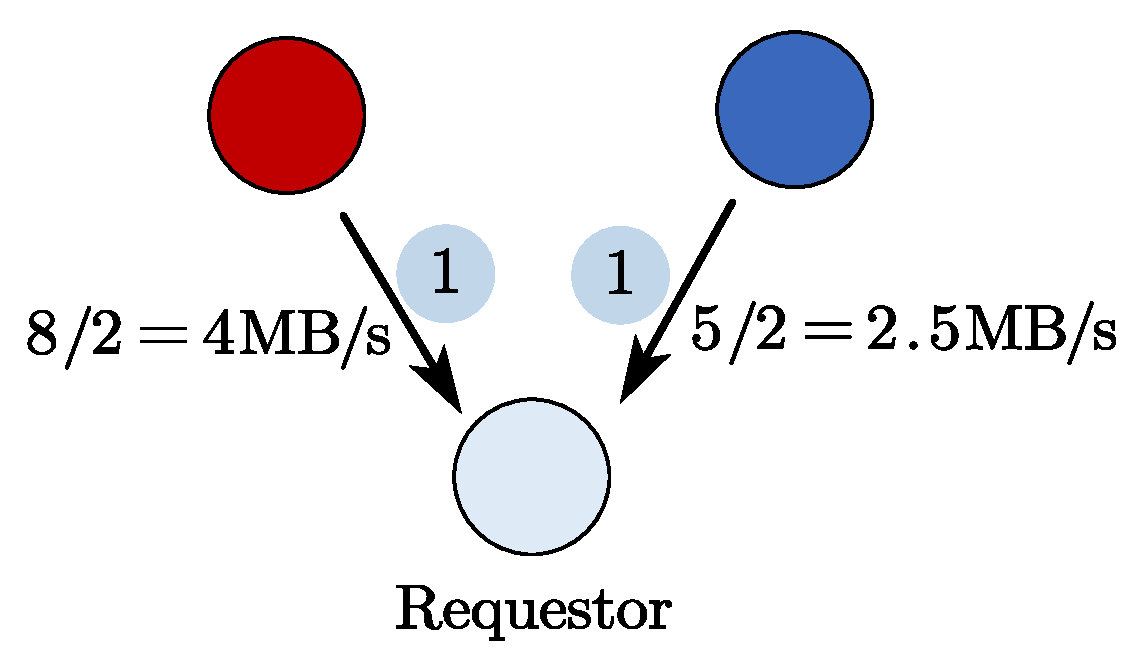
\includegraphics[scale=0.3]{figures/2.3-3.pdf}
            \caption{PPT: 通过并行传输绕过链路瓶颈}
            \label{fig:2.3-3}
    \end{subfigure}
    \begin{subfigure}[t]{0.4\textwidth}
            \centering
            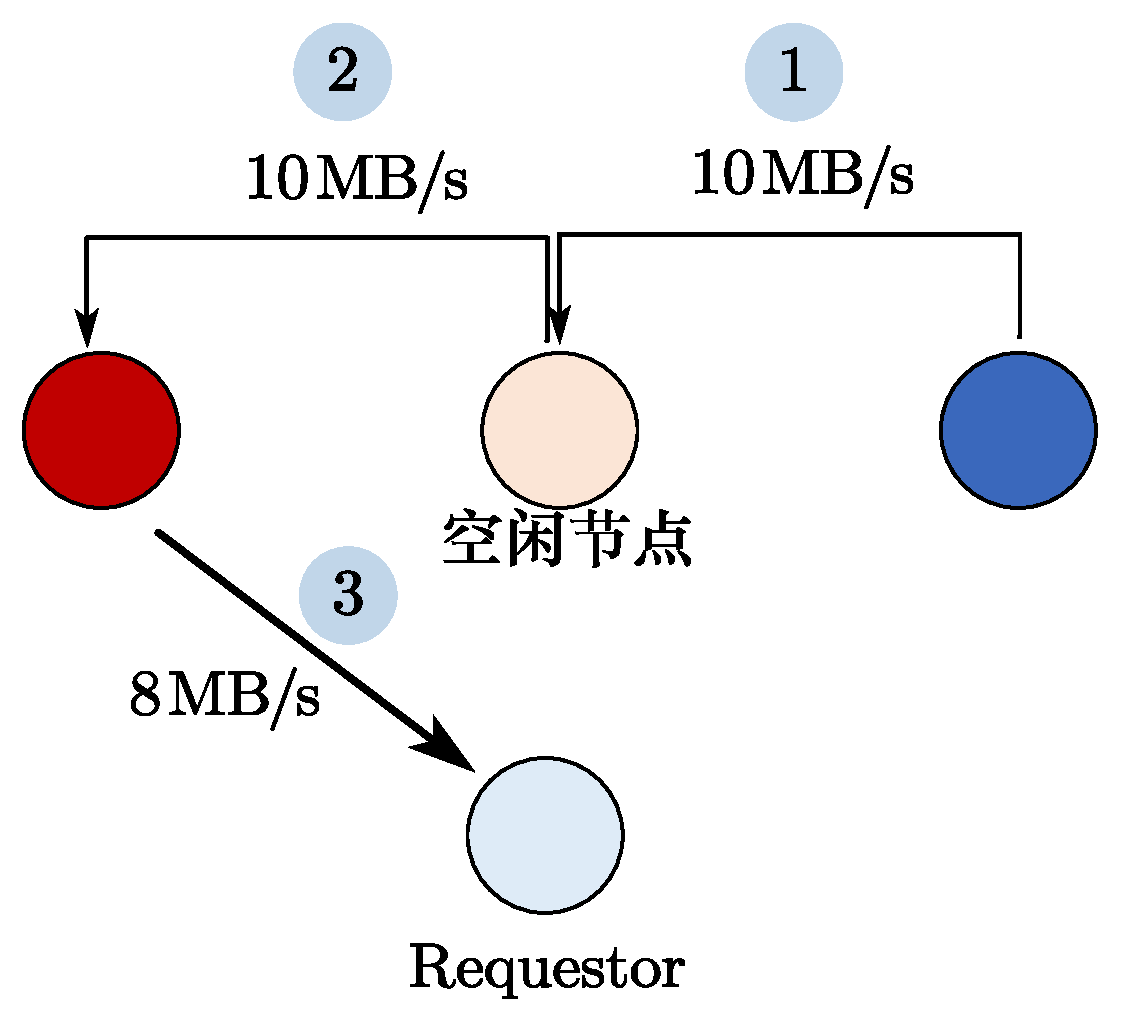
\includegraphics[scale=0.3]{figures/2.3-4.pdf}
            \caption{SMFRepair: 使用空闲节点绕过链路瓶颈}
            \label{fig:2.3-4}
    \end{subfigure}
    \caption{空闲节点可以绕过链路瓶颈,对于一个20MB的数据块而言,PPR、PPT和SMFRepair的修复时间分别为12.5s,8.0s,6.5s}
	\label{fig:2.3}
\end{figure}
针对快速修复技术,还有的研究聚焦于改善数据放置技术以提高修复速度。\citet{liu2020esetstore}提出了一种数据放置算法ESet来改善恢复性能,
他们通过理论分析说明ESet可以使用相应的配置实现I/O聚集情况下的快速单一故障修复,ESet是对现有修复技术的增强,最后他们通过在HDFS\cite{borthakur2008hdfs}
和Ceph\cite{weil2006ceph}中的实验
证明ESetStore的有效性,并将ESetStore进行了开源\footnote{开源地址:https://github.com/stevenlcj/ESetStore}。
此外,\citet{xu2020selectiveec}针对不同节点上工作负载的不均衡问题,定义了修复平行度DRP用来反映一个批次的重建任务中的负载平衡,
同时提出了一个平衡调度框架SelectiveEC,通过动态选择重建条带和平衡节点的上传下载带宽来改善单一修复任务的负载均衡。\citet{lin2021boosting}提出了一种快速修复调度框架RepairBoost,可以协助现有的线性纠删码和修复算法提高全节点的修复性能。
RepairBoost建立在三个主要技术上:
(1)总体修复,采用有向无环图来进行单块数据的修复;
(2)平衡修复流量,同时平衡上传和下载的修复流量;
(3)传输调度,精细地分配请求的数据块,使最未被占用的带宽达到饱和状态。
RepairBoost对于各种纠删码和修复算法,可以将修复速度提高35.0-97.1\%。

\section{基于带宽优化的数据修复技术}

目前实际的分布式存储系统经常独立地安排每个修复任务,鲜有考虑到任务彼此的影响。
这些分布式的修复任务共享着底层基础设施的网络、计算和存储资源,这就造成了数据流之间的干扰,导致系统资源利用率低下。
为了缓解这一问题,\citet{popa2013elasticswitch}提出了Elasticswitch,一种可以在各个服务器之间分配带宽的技术。
通过这一技术,将服务器的总带宽资源进行整合,可以为每个修复任务分配必要的网络带宽。此外,系统中主要有三种任务需要优化执行,
其中包括修复任务调度、调度数据的选择以及不同网段的后台修复任务的带宽分配。因此,\citet{li2018joint}提出了LSPT
(Linear Programming for Selected Tasks)在满足数据放置、网络拓扑结构以及带宽限制的条件下,最大限度地增加
满足时间限制的修复任务数。为了最佳地安排每个任务,LSPT共同解决了
(1)确定用于产生修复流量的纠删码块的选择问题,
(2) 在修复任务之间分配TOR交换机和聚合交换机带宽的带宽分配问题,以及
(3)根据最后修复时间限制安排任务的调度问题。

假设一个数据存储中心的一个聚合交换机连接着$u$个机架交换器(Top-of-Rack)。
$r$个存储节点($\mathcal{R}=\{1,2, \ldots, r\}$)放置在$u$个机架内($\mathcal{U}=\{1,2, \ldots, u\}$)并且每个
TOR交换器。同一个机架内所有的节点的修复流量不需要经过聚合交换机,而不同机架上的存储节点之间的流量则不需要经过两个
TOR交换机和聚合交换机。每份文件$i$用($n_i, k_i$)纠删码进行存储,保证为MDS(Maximum-Distance-Separable)码,确保
$n_i$中的任意$k_i$块可以重建文件$i$。此问题可以描述为,令$\mathcal{A}=\left\{A_{1}, A_{2}, \ldots, A_{m}\right\}$表示
为系统后台任务的集合,诸如备份,修复和数据再分配。对于每个任务$A_i$,相应地有关联参数包括数据块分发源$n_i$(表示为
$o_{i, 1} \in \mathcal{U}, o_{i, 2} \in \mathcal{U}, \ldots, o_{i, n_{i}} \in \mathcal{U}$),分发接收节点(表示为$p_{i} \in \mathcal{U}$),
需要获取的块个数$k_i$,每个块的大小$v_i$,任务开始时间$s_i$,以及任务的终止时间$d_i$。任务的开始时间和结束时间用秒作为单位,
满足$0 \leq s_{i} \leq d_{i}$。不失一般性,考虑带有时间段的系统,假设$y_{i, j}$为编码块的选择变量,例如$y_{i, j}=1$表示
块$j$被选择去执行任务$A_i$,而$y_{i, j}=0$则未被选中。既然块$k_i$必然被选择,则有

\begin{equation}
	\label{eq:2-1}
	\sum_{j} y_{i, j}=k_{i}, \forall i
\end{equation}

为了确定成功完成的任务数,使用二元变量$z_i$来进行表示,当$z_i=1$时任务$A_i$在时间限制内完成,否则未完成。
设$x_{t, i, j}$是在时间段$t$中分配给传输任务$A_i$的$j$块的数据流量的带宽,如果任务在最后期限$d_i$之前完成,
所有的$k$个块传输应该在$d_i$之间完成,即时间限制约束条件为:
\begin{equation}
	\label{eq:2-2}
    \sum_{t=s_{i}}^{d_{i}} x_{t, i, j} y_{i, j} \geq v_{i}, \text { if } z_{i}=1, \forall i, \forall j
\end{equation}

由于每个传输头尾对都有一个预先确定的路线,对于一个给定的任务集,用$RC_g$来表示跨越一个TOR或者聚合交换机$g$的任务或者
块的集合,即$(i,j)\in RC_g$如果任务$i$的块$j$的流量经过了交换机$g$。同样,$SC_h$是经过节点$h$的任务或者块集合。每个
TOR交换机有着容量的限制$CTA$且每个节点有着容量限制$CST$,因此有以下容量限制:

\begin{equation}
	\label{eq:2-3}
    \sum_{(i, j) \in R C_{g}} x_{t, i, j} y_{i, j} \leq C T A, \forall g, t
\end{equation}


\begin{equation}
	\label{eq:2-4}
    \sum_{(i, j) \in S C_{h}} x_{t, i, j} y_{i, j} \leq C S T, \forall h, t
\end{equation}

任务的目标就是要在基于纠删码的存储系统中最大化在时间截止内成功完成的修复任务数。可以看做是一个联合调度和优化问题:

\begin{equation}
    \begin{aligned}
    \label{eq:2-5}
    \max \quad & \sum_{i} z_{i}  \\
    \mbox{s.t.} \quad & \sum_{j} y_{i, j}=k_{i}, \forall i \\
    & \sum_{t=s_{i}}^{d_{i}} x_{t, i, j} y_{i, j} \geq v_{i} z_{i}, \forall i \\
    & \sum_{(i, j) \in R C_{g}} x_{t, i, j} y_{i, j} \leq C T A, \forall g, t \\
    & \sum_{(i, j) \in S C_{h}} x_{t, i, j} y_{i, j} \leq C S T, \forall h, t \\
    \mbox{var.} \quad & x_{t, i, j} \geq 0, y_{i, j} \in\{0,1\}, z_{i} \in\{0,1\}
    \end{aligned}
\end{equation}

其中式~\ref{eq:2-5}的第三行正好对应式~\ref{eq:2-2}任务成功时,即$z_i=1$。

% 在纠删码领域的大部分研究都集中在通过减少数据传输量(即修复带宽
% )来改善修复丢失的编码块时对网络的压力。目前已经提出了的一些编码结构,在进行修复时考虑到了网络拓扑结构的影响。

此外,还有部分研究集中在提升存储系统的适应动态网络变化的能力。\citet{li2010tree}提出了一个
基于Prim算法的树状拓扑感知修复方案,并构建了一个基于启发式方法进行修复的修复方案,考虑了修复过程中第二个存储节点丢失的情况。然而,这种方案
所造成的延迟通常情况下不满足系统的可靠性要求。其他相关研究集中在设计特定的网络拓扑结构,\citet{akhlaghi2010fundamental}根据读取节点的带宽开销,
将节点分为了两个集合,即“低廉”和“昂贵”两种集合。他们在这里引入了广义的再生码,并表示通过从“低廉”集合的节点中下载更多的块,可以减少修复故障节点
的所造成的开销。\citet{gaston2013realistic}为一个采用再生码的含有2个机架(rack)的系统提出了类似的模型,考虑了访问机架间和机架内数据的不同
访问成本和新加入节点的存储位置。\citet{hu2016double}引入了DRC(Double Regenerating Codes),最大限度地减少多机架数据中心的机架间流量。他们
提出了一个两阶段的再生修复程序,在修复之前,将存储在机架内的数据进行重新组合,实验结果显示,与传统的再生码相比他们的方案有着45.5\%的优化。
\citet{sipos2018network}通过引入一个通用的计算框架,提前计算不同的可能的修复方案的开销,从而使得纠删码的修复方案能够及时感知实时的网络环境,
做出相应的改变优化。

跨机架带宽往往会成为修复性能的瓶颈\cite{chowdhury2013leveraging,dean2004mapreduce},针对这个问题,
\citet{liu2020rack}提出了RPR(Rack-Aware Pipeline Repair Scheme)技术,一种机架感知的管道修复方案,
当存储系统发生单一故障或多个故障时,可以显著减少跨机架数据传输和总修复时间。
从负载均衡方面看,RPR对数据中心的有相应积极意义的。RPR技术由三个部分组成:
(1)校验数据块的放置,当校验块产生时,按照提高解码速度的规则放置在相应机架内;
(2)机架内部部分解码,在数据块传输到修复节点或机架之前,首先进行部分解码,这就减少了跨机架的数据传输,提高了负载平衡;
(3)跨机架管道修复,在部分解码之后,由修复管道算法决定内部机架和跨机架传输的顺序,以实现最佳的修复性能。实验结果表明,与传统修复方法相比,单节点修复RPR减少了
81.5\%的修复时间,与CAR\cite{shen2016reconsidering}相比修复时间减少了50.2\%,多节点修复总时间减少了64.5\%且机架间传输流量比传统RS码修复减少了50\%。

\citet{shen2020cluster}将问题的维度从机架感知扩大到集群感知,他们发现在大规模集群存储系统中,修复变得非常复杂,
同一集群内的节点之间因各种工作负载(如复制写入和MapReduce作业)而竞争的跨集群带宽往往被超额占用,
而且带宽消耗比集群内带宽消耗更加严重。因此,产生大量跨集群修复流量的修复任务(即跨集群搜索数据进行修复)将大大延长修复过程,并消耗更多的修复时间。
因此他们提出了ClusterSR\footnote{开源地址:https://github.com/shenzr/clustersr},一种智能感知集群带宽变化的分散修复技术,旨在最小化和平衡跨集群的修复流量。
ClusterSR首先验证系统的数据分布,并给出每个故障块的修复方案(指定读取同一条带的存活数据和存储修复数据的节点),
其主要目的是最小化跨集群修复流量。然后,ClusterSR将执行多个数据块的修复,从而使产生的跨集群上传和下载流量在各集群之间保持平衡。
ClusterSR是第一个在分散修复中考虑最小化和平衡跨集群上传和下载流量的工作。他们在Alibaba的ECS服务器上进行了大规模验证实验,ClusterSR可以减少
8.6-52.7\%的跨集群修复流量以及14.4-68.8\%的集群内修复流量。

\section{基于混合纠删码的数据修复技术}

大多数分布式存储系统倾向于采用恢复单一的纠删码来存储数据,但事实上存储系统中数据的访问频率并不相同,存在着冷数据与热数据之分。
改进方法便是采用恢复性能优秀的纠删码来存储热数据,存储开销低廉的纠删码来存储冷数据。例如,考虑LRC(6,3,2)和LRC(6,2,2),如果只使用其中任一单一编码都会
造成更高的存储开销和恢复成本。定义I/O开销为被读取的数据量和用户请求的数据量之间的差值,差值越小,则开销越小。如图~\ref{fig:2.2}所示,假设Client
请求$x_1,x_2$和$y_1$,但是$y_1$不可用,有很多种方法可以重建$y_1$,其中最高效的方法就是读取$p_x$和$y_2$来重建$y_1$。在这个例子中,读取的数据块
为4,且Client请求的的块数为3,所以I/O开销为$(4-3)=1$块。如图~\ref{fig:2.3}所示,假设Client在LRC(6,2,2)编码策略下
请求$x_1,x_2$和$y_1$,但是$y_1$不可用,所以读取$p_{xy}$来重建$y_1$。在这个例子中,读取的数据块
为3,且Client请求的的块数为3,所以I/O开销为$(3-3)=0$块。

\begin{figure}[tb!]
	\centering
	\begin{subfigure}[b]{0.8\textwidth}
		\centering
		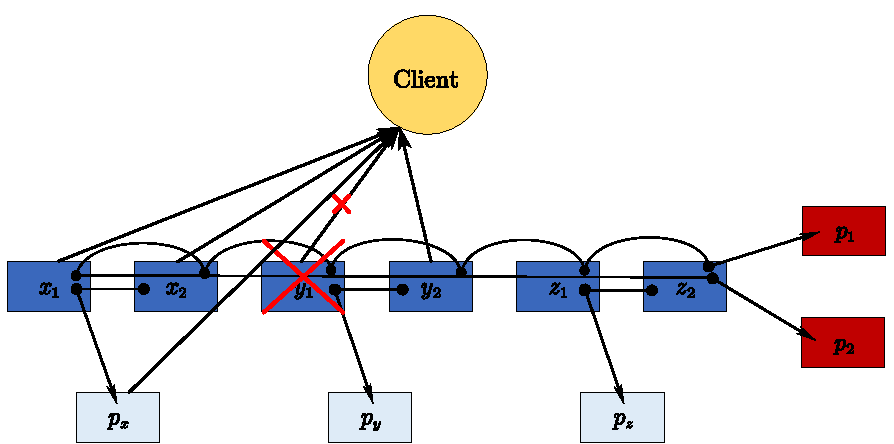
\includegraphics[scale=0.7]{figures/2.2.pdf}
		\caption{LRC(6,3,2),Client请求$x_1,x_2$和$y_1$且$y_1$处于丢失状态,所以Client访问$p_x$和$y_2$来重建$y_1$}
		\label{fig:2.2}
	\end{subfigure}
	\begin{subfigure}[b]{0.8\textwidth}
		\centering
		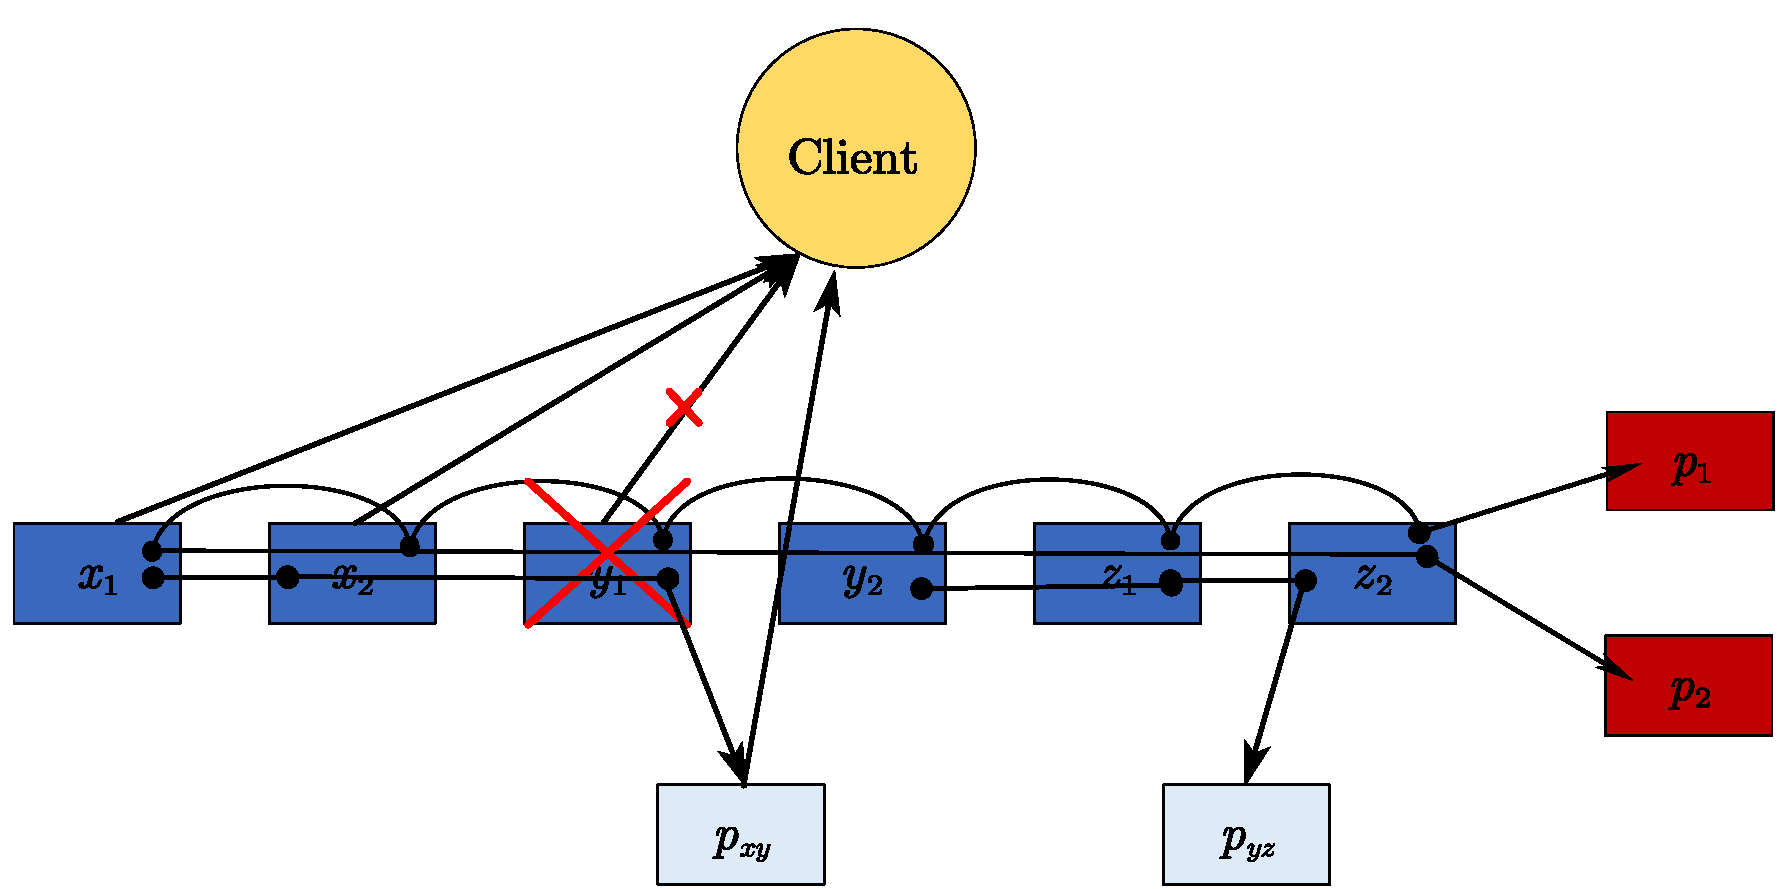
\includegraphics[scale=0.35]{figures/2.3.pdf}
		\caption{LRC(6,2,2),Client请求$x_1,x_2$和$y_1$且$y_1$处于丢失状态,所以Client访问$p_{xy}$来重建$y_1$}
		\label{fig:2.3}
	\end{subfigure}
	\caption{LRC(6,3,2)与LRC(6,2,2)不同重建方法}
	\label{fig:2.2-3}
\end{figure}


LRC(6,3,2)和LRC(6,2,2)的存储开销分别为(6+3+2)/6=1.83和(6+2+2)/6=1.67。
在相同的故障模式下,LRC(6,2,2)的重建成本和存储开销比LRC(6,3,2)低。
因此,在这种情况下,应该选择LRC(6,2,2)作为可靠性方案。
然而,上面描述的场景是一个特例,存储系统的存储要求比这个场景更复杂。
例如,一个应用程序可能一次读取一个或两个数据块,甚至不是一个完整的数据块。
在图~\ref{fig:2.2}和图~\ref{fig:2.2}中,他们只考虑了块$y_1$不可用的情况,但所有数据块都有相同的不可用概率。
受此启发,\citet{wei2018new}决定为分布式存储系统设计一种新的自适应编码选择方法,并用HDFS进行了验证,实验结果显示该方法将存储消耗减少了5\%,
修复带宽降低了22\%。
这个方法根据数据的访问特性来选择合适的LRC方案。
假设:用户请求的数据块是不可用的,
则可以计算出最小修复成本,并选择具有最小修复成本的LRC作为暖数据的存储方案。若某份数据在过去一段时间内的被访问量极低,
则冷数据编码模块就会启动MapReduce作业,用针对存储开销进行优化的RS码将LRC块转化为RS块,具体方法就是对于文件的每个编码条带的局部校验块$p_x,p_y,p_z$进行XOR运算,
从而生成一个新的全局校验块$p_0$,与原来的$p_1,p_2$组合并将$p_x,p_y,p_z$删除就将LRC转换为了RS码存储。
但是,对于这个自适应方案仍有几个问题需要解决。首先,冷数据随着时间的推移可能会转换成暖数据或者热数据,
应该针对这种情况配备对应的自适应的转换机制。
第二,没有考虑缺失的奇偶校验块,
尽管缺失的奇偶校验块并不直接影响修复性能,但会导致存储系统中I/O开销和网络带宽开销的增加,便间接地影响了修复性能。
第三,分布式存储系统有不同的故障模式,如块故障、磁盘故障和节点故障,这里只针对了块故障。


目前比较成熟和前沿的混合纠删码技术一般是含有两种纠删码,并对冷数据和热数据进行优化存储。
其中的技术包含了在两种纠删码进行高效切换的算法,在数据读取和写入过程中进行两种数据存储方式
的转换,此外还有采取优先级队列的方式来区别冷热数据并且配以相应的纠删码方案。
\citet{xia2015tale}采用两种纠删码来实现系统冗余,两种
编码属于同一种编码族,用Product Code作为快速码
(Fast code)为热数据来优化退化读和重建性能,用LRC
作为比较码(Compact code)针对冷数据来提供较为低
廉的存储消耗。具体实现方式如~\ref{fig:con-2.6}所示。


\begin{figure}[htbp]
	\centering
	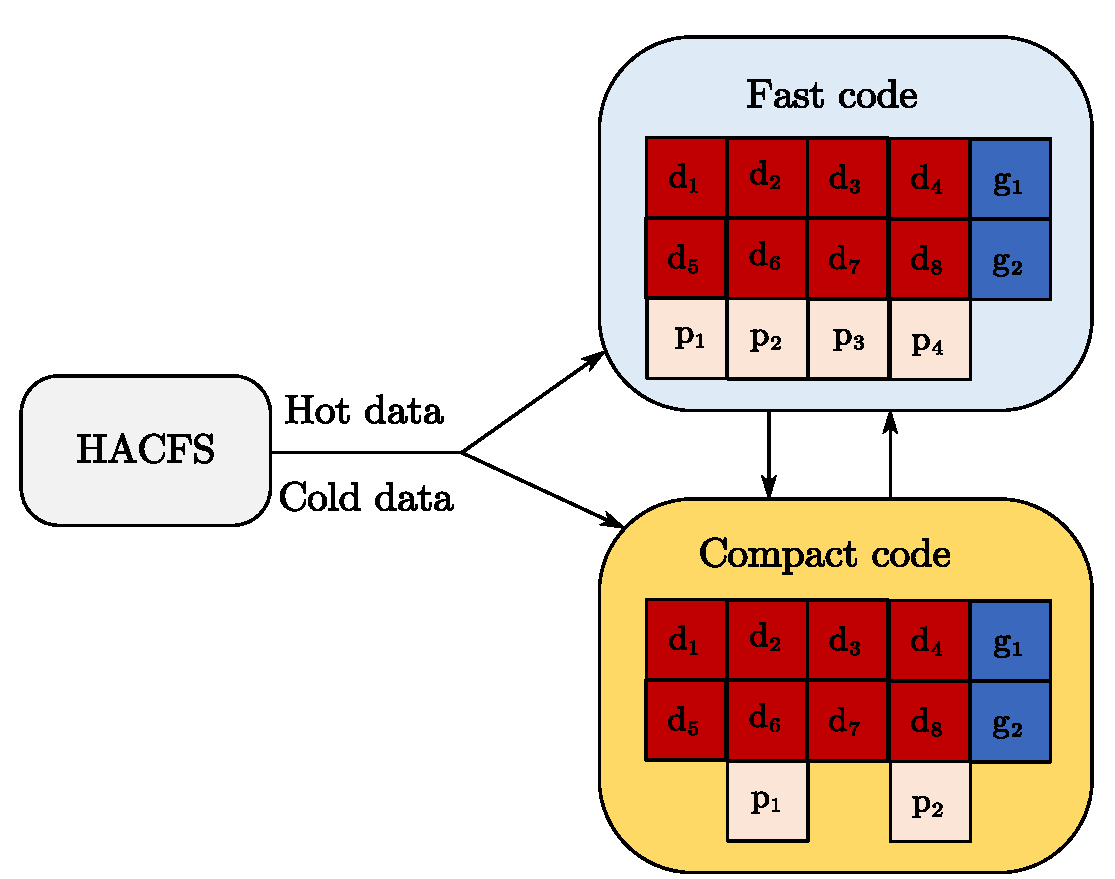
\includegraphics [scale=0.5]{figures/2.6.pdf}
	\caption{HACFS 混合纠删码的基本框架}
	\label{fig:con-2.6}
\end{figure}

HACFS的自适应编码模块管理着系统状态。系统状态跟踪模块记录着每个纠删码构建的数据文件的
以下文件状态:文件大小、最后修改时间、读取次数和编码状态。文件大小和最后修改时间是由HDFS维
护的属性,并由HACFS用来计算文件的总存储量和写入年龄。自适应编码模块还记录文件的读取次数,
此外一个文件的编码状态代表了它是否被复制了三份或是否已经被编码。文件状态可以在HDFS客户端对
该文件进行创建、读取或写入操作时被更新。


EC-Fusion由\citet{qiu2020ec}提出,他们将RS码和MSR(Minimum Storage
Regeneration)码结合到一起,其中RS码具有较低的
计算成本,为应用程序中的写请求提供了较低的开销。
而MSR码的修复过程中,单盘故障恢复的数据量和复
杂度较低,MSR在降低网络传输成本进行恢复方面具
有很大的优势,该技术将修复应用的速度提升了0.77倍,且修复时间降低了69.10\%。该方案包含三个主要特征:

\begin{enumerate}
    \item Code选择的调整,EC-Fusion将热数据划分
            为读取密集和写入密集型数据,然后又对数
            据的高低丢失风险做了相应的划分。冷数据
            或低风险数据采用RS进行编码,这保持了较
            高的存储效率,而且保证了良好的应用性能,
            特别是对于写入密集型I/O任务而言。对于
            具有高失效风险的读取密集数据,采取MSR
            编码可以节省大量的修复流量带宽,对应用
            程序的I/O产生很少的负面影响。
    \item 适应性规则,EC-Fusion采取现有的缓存算法
            (如LRU、LFU等)来识别热数据或冷数据。
            在EC-Fusion中,两个队列分别用于访问模
            式和故障特征,并且现有的缓存算法可以应
            用于这些队列中。其采用两个队列,第一个队
            列中的每个块包含了块ID、缓存命中次数,
            第二个队列的每个块包含块ID、缓存命中次
            数和编码方案的标志。
    \item Code的切换,在数据的属性保持动态变化的
            时候,如从热数据转换到了冷数据,高丢失
            风险数据变成了低风险数据。因为其本身数
            据保存时选择的编码方式不同,故相应的编
            码方式也要随着数据属性的变化而变化。即
            RS和MRS可以互相转换,其中MSR转
            RS如图~\ref{fig:con-2.7}所示。
\end{enumerate}

\begin{figure}[htbp]
	\centering
	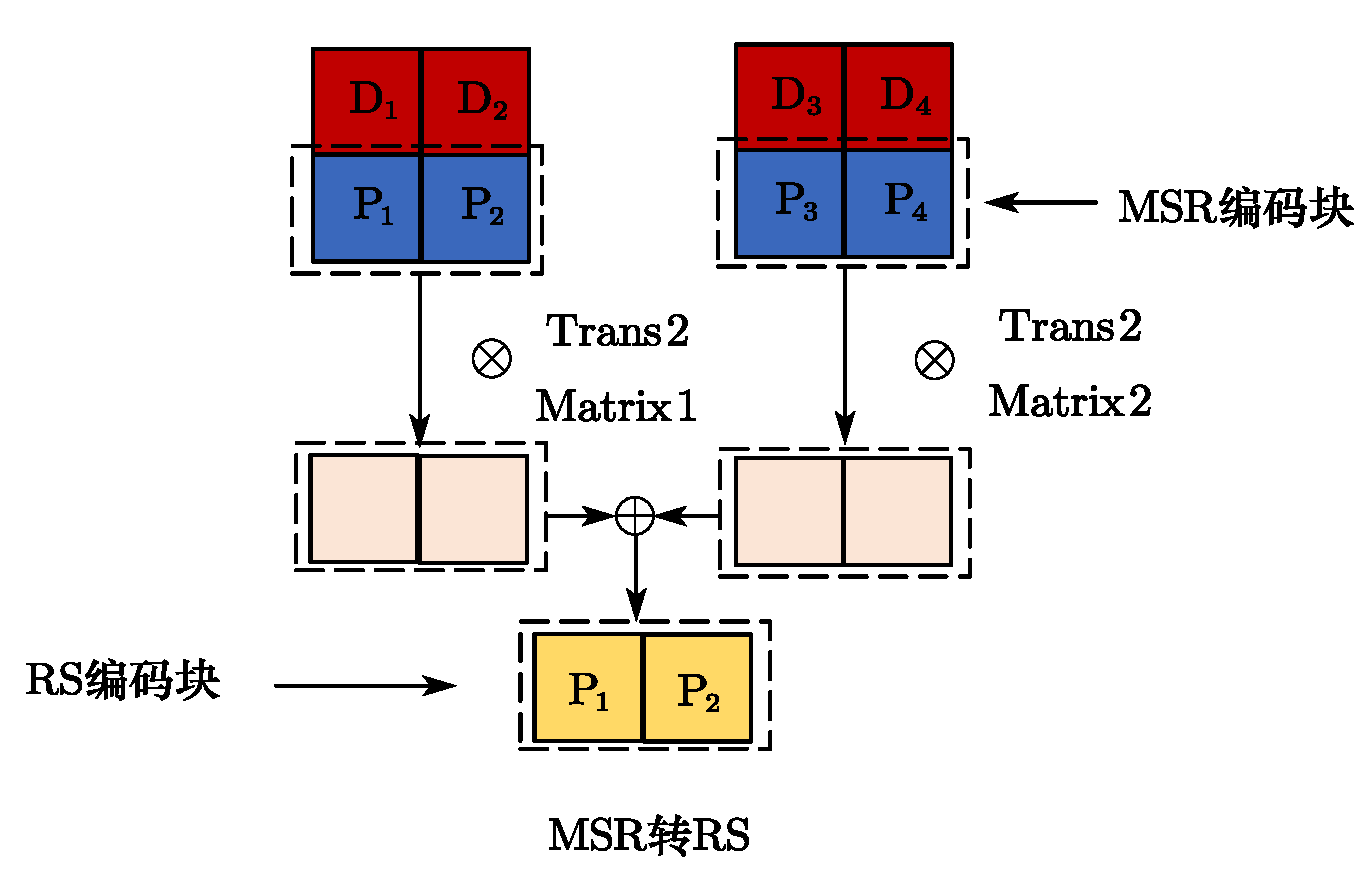
\includegraphics [scale=0.5]{figures/2.7.pdf}
	\caption{EC-Fusion中MSR转RS过程}
	\label{fig:con-2.7}
\end{figure}

\citet{wang2020adaptive}提出的这种策略使用LRC(Local
Reconstruction Code)来存储热数据 , 用HH码
(Hitchhiker)来存储冷数据,并且提出了相应的高效
转换算法平衡两者之间的网络带宽与计算性能的消
耗。HH码和LRC均为RS码的一种改进,在使用$(k,m)$HH码进行编码时,首先需要进行$(k,m)$RS码的编码,
再进行一系列Piggybacking框架中关于$g_i(a)$的异或运算;而在使用$(k,l,g)$LRC进行编码时,$g$个全局冗余块需要通过执行$(k,g)$RS码的
编码函数得到,而$l$个局部冗余块则只需要进行异或运算得到。另外$(k,m)$HH码中$g_i(a)$的计算,需要将$k$个数据块分为$(m-1)$组,
而$(k,l,g)$LRC中局部冗余块的计算,则需要将$k$个数据块分为$l$组。

从$(k,t-1,t)$LRC转换为$(k,t)$HH码时,首先将子条带$a$中的各局部冗余子块读取并传输到对应的全局冗余块所在节点,
并与该节点中子条带$b$的全局冗余子块进行异或运算,之后再将各局部冗余块删除即可。从$(k,t)$HH码转换为$(k,t-1,t)$LRC时,首先计算出所有局部冗余块,
之后再将其中子条带$a$中的局部冗余子块传到对应的全局冗余块所在节点,并与该节点中子条带$b$的全局冗余子块进行异或运算,
使得这些子条带$b$的全局冗余子块不再包含子条带$a$中的额外冗余信息$g_i(a)$。


\section{基于预先修复的数据修复技术}

由于磁盘故障预测技术的发展,磁盘故障的预测精度一般可以达到95\%\citep{botezatu2016predicting,li2014hard,mahdisoltani2017proactive,zhu2013proactive}。
在高度准确的磁盘故障预测潜力的加持下,\citet{shen2019fast}在通过假设拥有完备的预测技术精准预测除出STF(soon-to-fail)节点前提下,耦合两种修复方法,
即迁移与重建并提出FastPR算法,来对STF节点进行预先修复,其中(1)迁移,将STF节点上当前存储的数据块迁移到其他健康的节点上;(2)重建,
通过检索存储集群中所有健康节点的数据块来重建(或解码)STF节点的数据块,类似传统的反应式修复方法。
解决了纠删码中固有的带宽和I/O放大问题,而重建则利用了所有健康节点的总带宽资源。如图~\ref{fig:con-2.4}所示,假设系统使用的编码为RS(5,3),
即$n=5,k=3$,则一个条带
中有5个块包含了数据块和校验块,当前有7个节点($M=7$),其中6个健康节点和1个STF节点。
设$N_i$为第$i$个可用节点,$S_i$是要修复的STF节点的第$i$个块的条带。假设现在得到了一个STF节点的$c_m$和$c_r$的集合,
其中$c_m$为迁移的块的个数,$c_r$为重建的块的个数。对于这样的通常情况需要解决两个基本问题,
其一是在给定的通过重建修复的STF节点的$c_r$块中,需要确定从$k-c_r$个可用节点中检索出$k-c_r$个块,
可将$k-c_r$的搜索问题表述为一个二分图最大匹配问题。
其二是需要确定存储$c_m+c_r$个修复后的块。一般而言,将修复的块存储在$c_m+c_r$个现有的可用节点中
,这样就可以保持节点的容错性,即任何$n-k$个节点的故障都是可以容忍的,再次将选择$c_m+c_r$个可用节点表述为二分图最大匹配问题。


\begin{figure}[htbp]
	\centering
	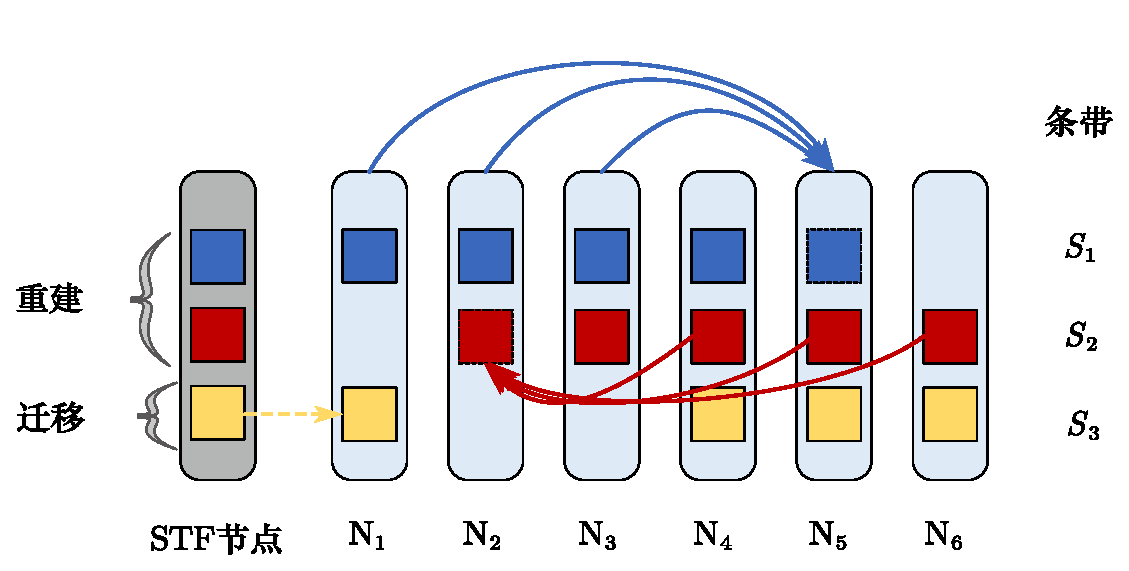
\includegraphics [scale=0.5]{figures/2.4.pdf}
	\caption{RS(5,3)编码系统的FastPR修复流程}
	\label{fig:con-2.4}
\end{figure}

根据访问频率,数据一般可以被区分为热、暖和冷数据
。一般来说,与热数据中的内容相比,暖数据的请求率较低,且可以通过历史访问数据和用户偏好从而预测数据访问热度,为了从用户角度减少访问时间,
\citet{cao2020popularity}融合了两种机器学习算法——预测和推荐,提出了新的一种预先修复技术POST。
针对暖数据,他们用一种独特的方式进行处理,以优化系统性能和存储空间的利用。
如图~\ref{fig:con-2.5}所示,为了使得故障的数据节点在响应I/O请求瞬时被重建,
他们采用了两种机器学习算法,其中包括用K-prototype聚类算法和基于贝叶斯的文本分析算法将文件进行聚类,
在数据重建过程中应用推荐算法优先修复访问量更高的文件。
他们提出的系统依赖于一个聚类机制,将文件分为多个集群,在每个集群中,文件都有类似的特征。
对于预测模块,通过跟踪历史数据的I/O访问,预测未来的访问热度较高的文件集,这个访问热度较高的文件集
反过来又提供了对可能接下来被访问的文件进行预测。
预测模块负责计算用户之间的相似性,从而设定要重建的数据块的优先级别。
实验结果表明,POST系统加快了并行存储系统的数据恢复,同时为在线用户保持了较高的数据访问性能。

\begin{figure}[tb!]
	\centering
	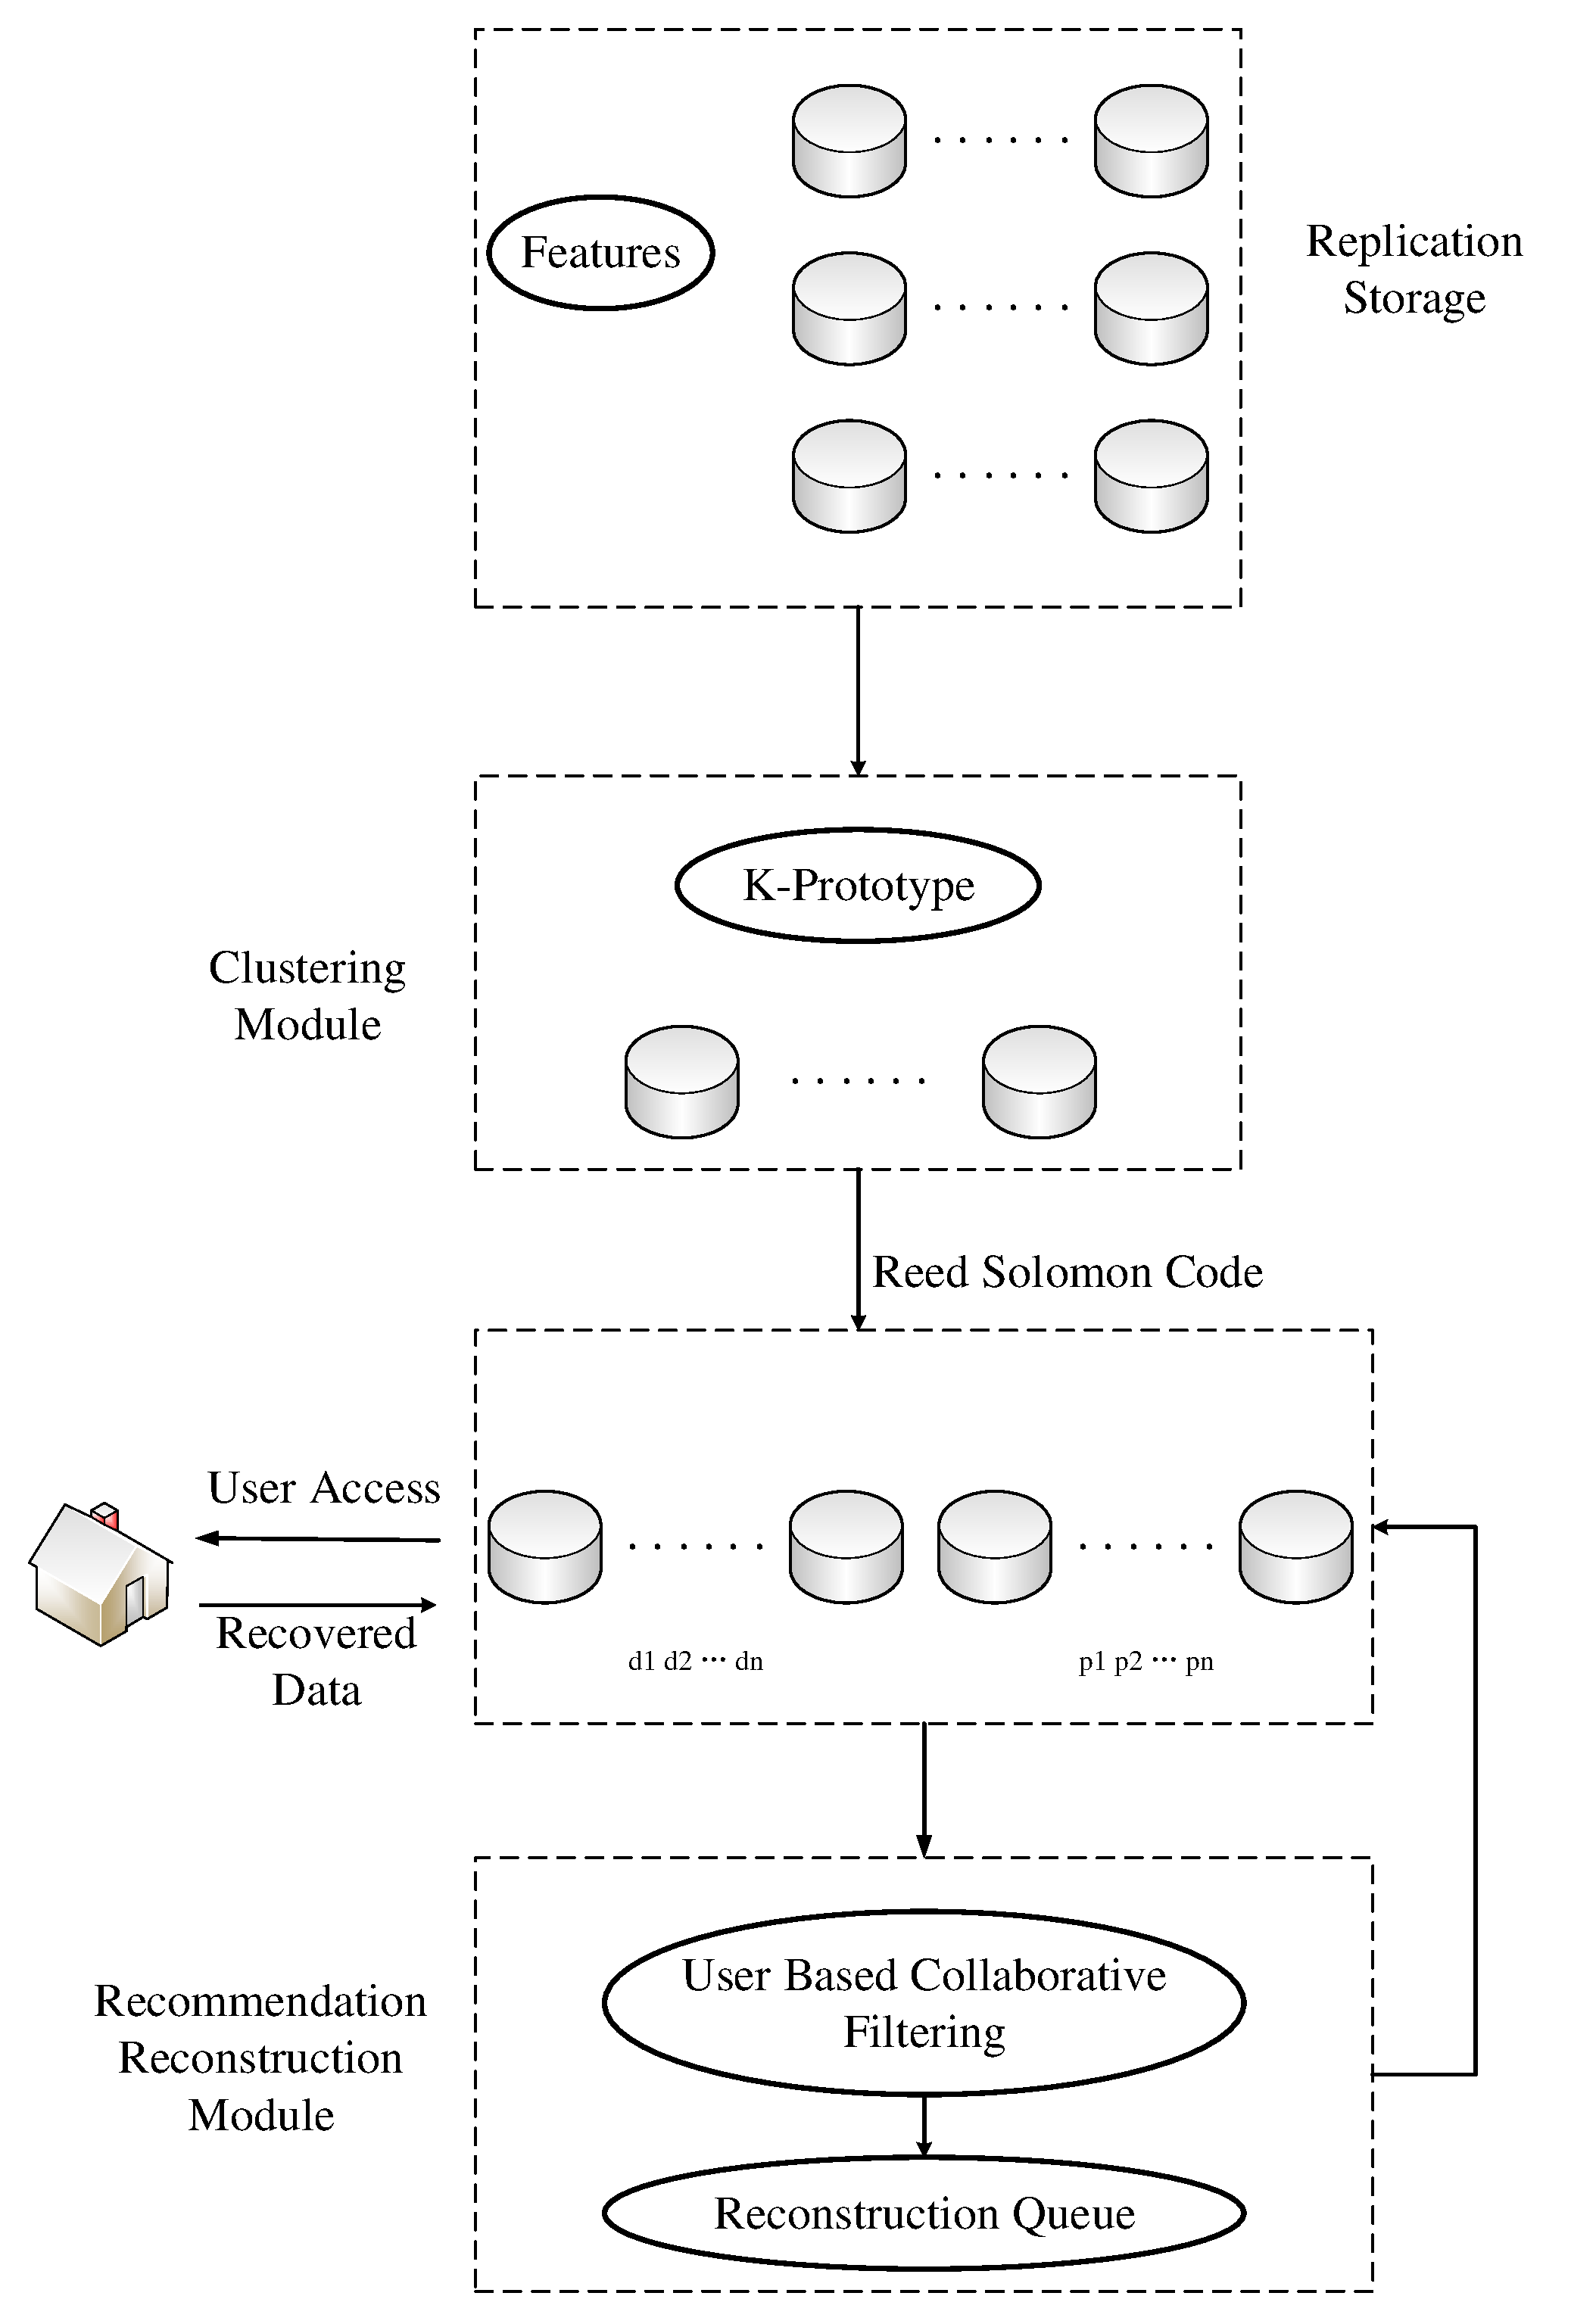
\includegraphics [scale=0.2]{figures/2.5.pdf}
	\caption{在POST的架构设计中,
    当带有特征的暖数据来自3倍复制的存储系统时,
    集群会通过K-Prototype算法将数据存储到基于纠删码的存储系统中,
    当用户在访问数据出现节点故障时,推荐系统会根据用户设置提供推荐列表,
    并为存储系统中的每个条带提供重建列表}
	\label{fig:con-2.5}
\end{figure}

此外,还有一些其他修复技术。针对纠删码数据块的随机分布问题,\citet{xu2020deterministic}提出了$D^3$(Deterministic Data Distribution),一种数据分布策略,其可以
在节点之间均匀地分发数据块和校验块,以及相应的基于$D^3$的高效数据修复算法。以往的研究很多忽略了数据块、校验块和文件之间的复杂关系,例如同时有5个块
在进行重建,且5个块属于5个不同的文件,那么此时5个文件都将无法访问。针对此问题,\citet{zeng2020fagr}提出了一种带有文件感知的图修复技术FAGR(File-aware Graph Recovery Scheme)
,从而提高重建过程中的文件修复速度。FAGR的思想建立一个文件、数据块、条带、校验块、
节点和文件访问频率之间的映射图,并从文件的角度引导数据修复过程。为了证明FAGR的有效性,他们
在集群中进行了一些数值分析和实验。结果表明,与典型的快速修复方法相比,FAGR将文件的平均响应时间减少了81.63\%,吞吐量提高了4.44倍。


\section{本章小结}
